\section{Component Selection} \label{component}

\subsection{Three-Phase Full Bridge Rectifier}
In the first stage, we need a three-phase rectifier. For the three-phase rectifier, we decided to use a three-phase bridge diode similar to the \cite{three-phase_bridge} in Figure \ref{fig:bridge} to rectify the signal with the addition of an appropriately sized capacitor. Necessary constraints are given in the Table \ref{tab:ratings_diode}. If we struggle on the three-phase rectifier, we can also consider turning back to the single-phase version of the topology.

\begin{table}[ht]
    \centering
        \begin{tabular}{|c|c|c|}
        \hline
         Peak Voltage   & Peak Current    & Voltage Ripple  \\ 
        \hline
         210 Vpeak      & 31A             & 20Vpp           \\
        \hline
        \end{tabular}
    \caption{Ratings obtained from the Simulations}
    \label{tab:ratings_diode}
\end{table}

\begin{figure}[ht]
    \centering
    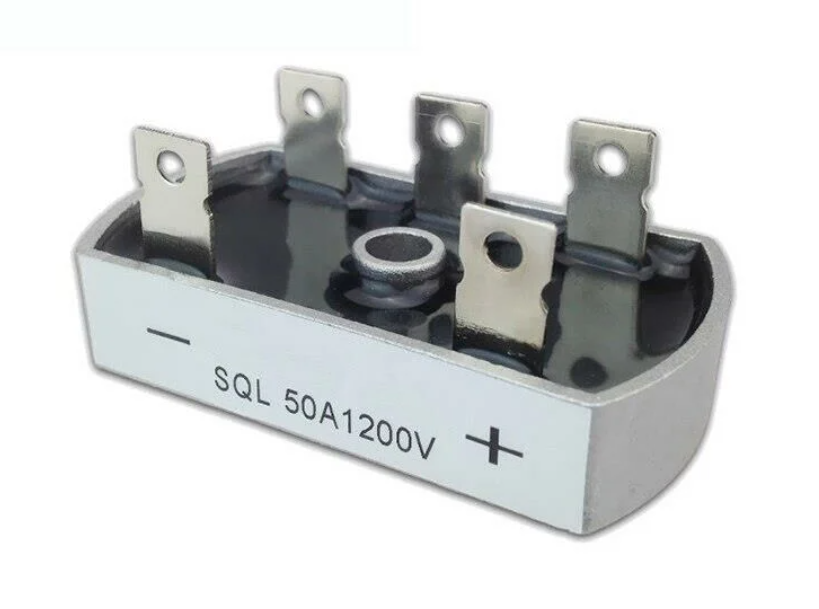
\includegraphics[width=0.4\textwidth]{matlab/bridge_diode.png}
    \caption{Three-phase Full Bridge}
    \label{fig:bridge}
\end{figure}

\subsection{MOSFET Selection}
In MOSFET Selection, transients and peak values play an important role during the switching instants. For conduction modes, continuous current is considered.

\begin{table}[ht]
    \centering
        \begin{tabular}{|c|c|c|}
        \hline
         Peak Voltage   & Peak Current    & Continuous Current  \\
         \hline
         210 V          & 30A             & 10A          \\
        \hline
        \end{tabular}
    \caption{Ratings obtained from the Simulations}
    \label{tab:ratings_DC}
\end{table}

As the voltage rating of the MOSFET increases, the $R_{ds,on}$ resistance of the MOSFET increases. We decided to keep our MOSFETs around the boundaries because we use five of them. 

\begin{table}[ht]
    \centering
        \begin{tabular}{|c|c|c|}
        \hline
         Peak Voltage   & Peak Current    & Continuous Current  \\ 
         \hline
         300 V          & 50A          & 30~40A          \\
        \hline
        \end{tabular}
    \caption{Intended Ratings for MOSFETS}
    \label{tab:ratings_MOS}
\end{table}
There was not enough time to do wide market research for the component selection. Therefore only a few models can be detected initially. Table \ref{tab:selected_MOS} shows some of the possible options. If we can find a model that suits better to our design than the ones given in Table \ref{tab:selected_MOS}, in terms of efficiency, cost and availability, we will consider choosing that model for our design. 

\begin{table}[ht]
    \centering
        \begin{tabular}{|c|c|c|c|c|}
        \hline
         Model   & $V_{ds}$ Voltage(V)    & Continuous Current(A) & $R_{ds,on}(m\Omega)$ & Peak Current(A) \\ 
        \hline
        
         FDAF62N28       &280           &36              &51     &144\\
         FDAF75N28      &280           &46             &51      &184\\
         FDB38N30U       &300           &38             &120     &152\\
         AUIRFP4409     &300            &36             &69     &156\\
         IXFP38N30X3   & 300           & 36            & 34     & 60A\\
         FDA38N30       &300           &38             &70       &150\\ 
         IXTQ52N30P   & 300           & 52            & 66     & 150A\\
         IPB60R060P7ATMA1 &600         &48             &60       &151A\\
           
        \hline
        \end{tabular}
    \caption{Some of the Selected MOSFETs}
    \label{tab:selected_MOS}
\end{table}